\chapter{Лекция 1: Темы теории струн}

\lectureoverview{Вызов редукционизму становится острее благодаря бозонизации в \(1+1\) измерениях, электрической--магнитной дуальности, D-бранам, переходам при сильной связи, эмерджентной геометрии и комбинаторному ландшафту струнных вакуумов. Одна и та же физическая система может допускать радикально разные элементарные описания; то, какое из них выглядит простым, зависит от константы связи и геометрии.}

\section{Редукционизм, сложность и вопрос о простоте}

Сасскинд начинает с намеренно знакомого философского лозунга: большие вещи состоят из маленьких, а маленькие — из еще меньших. Затем он добавляет более амбициозную версию той же идеи, ту, которая действительно важна для фундаментальной физики: по мере спуска к более глубоким слоям объекты должны становиться не только меньше, но и проще. Его метафора такова: дома сделаны из кирпичей, и никто не примет дом за кирпич. Кирпич меньше, но он и проще.

Первый шаг лекции — сопоставить это ожидание с реальным состоянием физики частиц. Если бы редукционизм действительно приносил возрастающую простоту в этом сильном смысле, можно было бы ожидать, что современная физика элементарных частиц уже будет устроена экономно. Вместо этого Сасскинд подчеркивает, что еще до включения квантовой гравитации учет уже выглядит громоздким. В лекции приводятся грубые подсчеты, но эта грубость и есть часть замысла:
\begin{equation}
\begin{aligned}
N_{\mathrm{species}}&\sim 75,\\
N_{\mathrm{independent}}&\sim 10\text{--}20,\\
N_{\mathrm{parameters}}&\sim 20.
\end{aligned}
\end{equation}
Но и этим история не заканчивается. Стандартная модель не содержит гравитации, не объясняет темную материю, не дает дополнительной структуры, необходимой для инфляции, и несет в себе серьезную проблему тонкой настройки. Добавление обычных механизмов исправления лишь увеличивает число параметров. Примером в лекции служит суперсимметрия. Во время этой лекции многие физики надеялись, что Большой адронный коллайдер обнаружит суперпартнеров; Сасскинд подчеркивает, что соответствующее расширение ввело бы более ста дополнительных параметров, а не сразу упростило бы эту схему учета. Схематически его мысль такова
\begin{equation}
N_{\mathrm{parameters}}^{\mathrm{extended}} \sim 200.
\end{equation}
Эти числа намеренно грубы и имеют исторический характер. Они служат аргументом в пользу того, что более глубокое описание не обязано выглядеть проще на уровне перечня частиц и измеряемых констант.

Это количественное возражение — еще не главный тезис Сасскинда. Это лишь прелюдия. Более глубокое утверждение, и именно оно ведет дальнейшую часть лекции, состоит в том, что современная квантовая теория поля и теория струн, вообще говоря, не дают очевидного основания для единственного, не зависящего от константы связи различия между кирпичами и домами. Следующие примеры выбраны так, чтобы показать, что сам смысл ``элементарного'' может зависеть от того, какие переменные оказываются эффективными.

\section{Бозонизация: первый подрыв идеи фиксированной фундаментальности}

Первый теоретический пример Сасскинда взят из квантовой теории поля в \(1+1\) измерениях: одно пространственное измерение и одно временное. Он сразу оговаривает, что не будет подробно выводить эту эквивалентность; смысл не в формальном доказательстве, а в концептуальном уроке.

Начинают с теории поля фермионов. Фермионное поле обозначается \(\psi\). Два близко расположенных фермиона могут образовать бозонный композит, и соответствующее бозонное поле обозначается \(\phi\). На первый взгляд иерархия кажется ясной: \(\psi\) первично, тогда как \(\phi\) — составная или эффективная переменная. В лекции бозон вводится именно так, как поле, создающее связанные пары фермионов.

Однако было обнаружено, что ту же теорию можно переписать, исходя из противоположной отправной точки. Можно начать с бозонного поля \(\phi\), и тогда фермион больше не возникает как точечный компонент. Вместо этого он появляется как кинк бозонного поля — протяженная конфигурация, в которой \(\phi\) гладко интерполирует между двумя асимптотическими значениями. Минимальное математическое содержание лекции состоит в следующей асимптотической структуре:
\begin{equation}
\phi(x\to -\infty)=\phi_-,
\qquad
\phi(x\to +\infty)=\phi_+.
\end{equation}
Удобный схематический представитель имеет вид
\begin{equation}
\phi(x)\approx \frac{\phi_++\phi_-}{2}
+
\frac{\phi_+-\phi_-}{2}\tanh\!\left(\frac{x}{\ell}\right),
\end{equation}
где \(\ell\) — ширина переходной области.

\editorialnote{Профиль с гиперболическим тангенсом — стандартный гладкий представитель кинка, изображенного в лекции, а не формула, выведенная в ней. Точный словарь бозонизации зависит от модели; концептуально важно здесь то, что фермионное возбуждение и топологический солитон бозонного поля меняются ролями.}

Аналогия с ремнем в лекции достаточно точна, чтобы ее стоило сохранить. Плоский ремень без перекрута — это конфигурация без кинка. Если повернуть один конец на \(2\pi\), вдали ремень возвращается к той же локальной ориентации, но между этими областями он должен пройти через протяженную перекрученную область. Эта перекрученная область и есть кинк. В бозонном описании фермион представлен именно таким протяженным объектом.

Эта мысль становится резче, как только вводится константа связи. В этом примере Сасскинд обозначает ее \(G\). Утверждается не то, что эти два описания как-то расплывчато связаны, а то, что их эффективность зависит от режима параметров:
\begin{align}
G \ll 1
&\Rightarrow
\ell\text{ small, tight kink; }\psi\text{ efficient},\\
G \gg 1
&\Rightarrow
\ell\text{ large, broad kink; }\phi\text{ efficient}.
\end{align}
При малом \(G\) кинк компактен, и именно фермион выглядит простым объектом. По мере роста \(G\) кинк расширяется, и фермион становится менее точечноподобным. Тогда более экономичными оказываются бозонные переменные.

\paragraph{Схематическое правило перехода.}
\begin{enumerate}
\item Начните с фермионной теории, описываемой \(\psi\).
\item Выделите бозонные композиты, описываемые \(\phi\).
\item Перепишите ту же теорию целиком через \(\phi\).
\item В бозонном описании фермион снова возникает как кинк ширины \(\ell\).
\item При \(G\ll 1\) \(\ell\) мало, и самым простым оказывается фермионное описание.
\item При больших \(G\) \(\ell\) растет, и самым простым становится бозонное описание.
\end{enumerate}

Это первый явный контрпример к фиксированной картине ``домов и кирпичей''. Главная мысль лекции не просто в том, что существуют составные объекты, а в том, что то, что считается элементарной переменной, может меняться при изменении константы связи.

\section{Электрический заряд, магнитные монополи и режимы слабой и сильной связи}

Затем Сасскинд спрашивает, возникает ли аналогичная история в более привычной физике частиц. Примером служит электрический заряд в сравнении с магнитным монополем. Обычная заряженная частица, например электрон, в этой терминологии является электрическим монополем: локализованным источником электрического поля. Магнитный монополь вводится через аналогию со стержневым магнитом. Если бы удалось каким-то образом изолировать конец стержневого магнита без невидимого соединительного стержня, силовые линии выглядели бы в точности как у электрического заряда, только магнитные, а не электрические.

Существенным управляющим параметром является постоянная тонкой структуры \(\alpha\). В лекции Сасскинд эвристически трактует ее как квадрат электрического заряда:
\begin{equation}
\alpha \sim e^2.
\end{equation}
Он также дает грубое операционное толкование: она измеряет, насколько легко электрон излучает, и суммирует эту силу, говоря, что ускоренный электрон в соответствующем смысле излучает порядка ``\(1/100\)'' фотонов. В грубом численном языке самой лекции,
\begin{equation}
\alpha \approx 10^{-2}.
\end{equation}
Это не следует понимать как точную конвенцию; это педагогический способ выразить, что электрический заряд слаб.

\editorialnote{Связь слабой--сильной связи имеет точный прообраз в квантовании Дирака. В одном распространенном соглашении электрический и магнитный заряды удовлетворяют \(e g_m=2\pi n\). Следовательно, слабой электрической связи соответствует сильная магнитная, хотя точные численные множители и защищенные соотношения для масс зависят от теории.}

Когда \(\alpha\ll 1\), электрон является простым объектом. Его электрическое поле слабо, облако поляризации вакуума разрежено, и он выглядит почти точечным. Магнитный монополь тогда противоположен ему: его поле огромно, его окрестность резко искажена, и сам он протяжен, сложен и тяжел. Сасскинд резюмирует ситуацию именно в этом стиле слабой--сильной связи:
\begin{equation}
\begin{aligned}
\alpha \ll 1
&\Rightarrow \text{simple electron;}\\
&\phantom{\Rightarrow{}}\text{heavy, extended monopole},\\
\alpha \gg 1
&\Rightarrow \text{simple monopole;}\\
&\phantom{\Rightarrow{}}\text{heavy, structured electron}.
\end{aligned}
\end{equation}
В лекции не выводится формула массы монополя. В ней нет необходимости. Суть здесь качественная. По мере увеличения \(\alpha\) поле электрона усиливается и его структура разрастается, тогда как монополь сжимается и становится легче. При значениях, намного превышающих единицу, удобное описание меняется местами: прост монополь, а электрон сложен.

Это полевотеоретическая версия прежнего урока бозонизации. Различие между фундаментальным и составным не является абсолютным. Оно зависит от константы связи.

\begin{classroomqa}
\audiencequestion{Если редукционизм не является надёжным ориентиром, почему физики полагаются на математический анализ, который, по-видимому, делит систему на сколь угодно малые части? \lecturetimestamp{00:21:21}}
\lecturerresponse{Математический анализ утверждает гладкое изменение; он не определяет фундаментальные объекты теории. Квантовые поля флуктуируют на всех масштабах расстояния, порождая бесконечную иерархию, а не некоторый последний гладкий слой, на котором можно было бы раз и навсегда решить, что является элементарным.}
\end{classroomqa}

Обмен репликами продолжается предположением, что эта иерархия напоминает фрактал. Сасскинд принимает аналогию, а затем уточняет её: квантовые поля флуктуируют на всех масштабах и потому никогда не являются гладкими в классическом смысле. Эта чрезмерная изменчивость — часть того, что делает квантовую теорию поля математически трудной; обычный математический анализ приходится применять к перенормированным величинам, а не к наивно гладкому микроскопическому полю.

\section{Струны, D-браны и возвращение слабой--сильной дуальности}

Следующий переход в лекции намеренно наивен. Если теория струн должна быть теорией фундаментальных составляющих, то ответ, конечно, должен быть прост: этими составляющими являются струны. Сасскинд открыто формулирует это ожидание, а затем посвящает следующую часть лекции тому, чтобы его разобрать.

\subsection{Почему струны — не вся история}

Первая трудность состоит в неизбежном присутствии D-бран. D\(p\)-брана — это \(p\)-мерный объект, на котором могут оканчиваться струны. Буква \(D\) происходит от граничных условий Дирихле, но имя гораздо менее важно, чем роль: эти объекты входят в теорию и не могут быть отброшены. Это не факультативные украшения.

Простейшие примеры таковы:
\begin{itemize}
\item D0-брана, которая является точечным объектом,
\item D1-брана, или D-струна, которая является струноподобным объектом,
\item F-струна, обычная фундаментальная струна.
\end{itemize}
D0-брана — это тяжёлый точечный узел, на котором может оканчиваться сколь угодно много F-струн. D1-брана — тяжёлый кабелеобразный объект, гораздо более толстый и обладающий гораздо большей массой на единицу длины, чем F-струна, но также служащий местом, где могут оканчиваться F-струны. При слабой связи лекция не представляет эти объекты как в равной мере элементарные альтернативы. D-браны вводятся как тяжёлые, структурированные, на вид составные объекты, которые теория, тем не менее, навязывает нам.

\editorialnote{Используемая в этой части лекции теория с нечётными бранами — это теория струн типа IIB. Её стабильные D-браны имеют нечётную пространственную размерность, включая D1- и D3-браны. Сасскинд откладывает эти названия, поскольку непосредственная тема — схема дуальности, а не таксономия.}

\paragraph{Обозначения.}
Сасскинд несколько вольно использует \(G\) и \(g\) в разных частях лекции. Здесь \(G\) зарезервировано для примера с бозонизацией, тогда как \(g\) обозначает струнную константу связи.

Струнная константа связи \(g\) определяется операционально, а не аксиоматически. Это параметр, измеряющий вероятность того, что флуктуирующая струна расщепится и образует дочерние струны. Поэтому Сасскинд напрямую сравнивает её с ролью \(\alpha\) в КЭД. В лекции также делается пауза, чтобы отождествить натяжение с энергией на единицу длины:
\begin{equation}
T=\frac{E}{L}=\frac{M}{L}.
\end{equation}

Для F-струны и D-струны стандартные формулы для натяжения делают сравнение слабой--сильной связи явным:
\begin{equation}
T_{\mathrm{F1}}=\frac{1}{2\pi\alpha'},
\qquad
T_{\mathrm{D1}}=\frac{1}{2\pi\alpha' g_s},
\qquad
\frac{T_{\mathrm{D1}}}{T_{\mathrm{F1}}}=\frac{1}{g_s}.
\end{equation}
\editorialnote{Эти формулы для натяжения задают общепринятую нормировку, стоящую за качественным сопоставлением кабеля и нити в лекции. Это редакторское добавление; в самой лекции используется только зависимость от константы связи.}

\subsection{F-струны и D-струны}

Затем история слабой--сильной связи повторяется на языке струн. При малой связи F-струна легка, тонка и близка к исходному интуитивному образу фундаментального объекта. D-струна толста, тяжела и наполнена структурой из F-струн. По мере роста связи F-струна легче расщепляется; облако дочерних струн вокруг неё разрастается, и она становится тяжелее и сложнее. В то же время D-струне всё труднее испускать ставшие теперь тяжёлыми F-струны, так что окружающая её структура редеет, и она становится легче и более нитевидной. Поэтому схема слабой--сильной связи в лекции такова
\begin{align}
g \ll 1
&\Rightarrow
\begin{gathered}
\text{F-string light and thin;}\\
\text{D-string heavy and structured},
\end{gathered}\\
g \sim 1
&\Rightarrow
\text{F-string and D-string comparable},\\
g \gg 1
&\Rightarrow
\begin{gathered}
\text{D-string light and thin;}\\
\text{F-string heavy and structured}.
\end{gathered}
\end{align}
Сасскинд замечает, что вблизи \(g\sim 1\) эти два описания перестают чётко различаться. За этой точкой они фактически меняются ролями. Это струнно-теоретическая версия обмена электрон--монополь, и её общепринятое название — S-дуальность.

Тот же обмен можно проследить и после того, как струна замыкается в петлю. При слабой связи маленькая петля F-струны является лёгким частицеподобным возбуждением, тогда как соответствующая петля D-струны тяжела и сложна. При сильной связи их роли меняются: петля D-струны становится лёгким описанием, и среди возникающих при этом лёгких возбуждений замкнутой струны есть гравитон. Этот пример в лекции нужен для того, чтобы настоять: даже тождество знакомой частицы может зависеть от того, с какой стороны дуальности ведётся описание.

Лекция продвигает эту мысль ещё на один шаг. В идеализированной теории константа связи — не просто число, которое можно выставлять вручную; она ведёт себя как поле. Схематически,
\begin{equation}
g = g(x).
\end{equation}
Поэтому в разных областях пространства могут быть предпочтительны разные дуальные описания. В одной области лёгкими переменными являются F-струны; в другой — D-струны. Между ними ничто не является особенно простым. Вот почему, с точки зрения Сасскинда, теория струн не восстанавливает простую редукционистскую картину. Она радикализует эту неоднозначность.

\editorialnote{В пертурбативной теории струн локальная константа связи задаётся дилатоном, \(g_s(x)=e^{\Phi(x)}\). Поэтому запись \(g=g(x)\) — не просто аналогия, хотя реалистические компактификации, как правило, порождают потенциал, который ограничивает такие вариации.}

\begin{classroomqa}
\audiencequestion{Если бы константа связи менялась настолько, что в другой области D-струны становились бы легче F-струн, повлияло бы это изменение на наблюдаемые спектры? \lecturetimestamp{00:34:15}}
\lecturerresponse{Да. Это одна из причин, по которым обсуждаемую точно симметричную, математически контролируемую модель нельзя напрямую отождествить с нашим миром. Её уроки касаются того, на что способны непротиворечивые квантовые теории, а не буквального спектра природы.}
\end{classroomqa}

\begin{classroomqa}
\audiencequestion{Существует ли аналогичное дуальное описание для D2-браны? \lecturetimestamp{00:34:39}}
\lecturerresponse{Да, но это не ещё один обмен по типу D-струны. Случай чётных бран приведёт к мембранной интерпретации и к дополнительному пространственному измерению; это и есть следующая конструкция.}
\end{classroomqa}

\begin{classroomqa}
\audiencequestion{Объясняет ли большая вероятность расщепления струны возросшую внутреннюю сложность? \lecturetimestamp{00:34:53}}
\lecturerresponse{Да. Чтобы сделать механизм наглядным, вернёмся к КЭД: электрон испускает фотоны, фотоны флуктуируют в заряженные пары, а эти заряженные линии снова излучают. При увеличении связи эта иерархия становится менее разреженной.}
\end{classroomqa}

\subsection{Возвращение к квантовой электродинамике в ответ на вопросы}

Затем студент спрашивает, означает ли большая вероятность расщепления просто более сложную структуру ``выше по иерархии''. Сасскинд отвечает, возвращаясь к квантовой электродинамике и снова рисуя мировую линию электрона. Это возвращение важно: оно показывает, что история со струнами — не изолированная диковина, а ещё один случай той же схемы слабой--сильной связи.

\begin{figure}[htbp]
\centering
\begin{tikzpicture}[scale=1.0]
\draw[->] (-1.2,0) -- (3.7,0) node[right] {space};
\draw[->] (0,-0.2) -- (0,4.3) node[above] {time};

\draw[line width=0.9pt] (0,0.2) -- (0,4.0);
\node[left] at (0,3.55) {\(e^{-}\)};

\draw[line width=0.8pt] (0,1.0) -- (0.18,1.08) -- (0.36,0.92) -- (0.54,1.10) -- (0.72,0.94) -- (0.90,1.12) -- (1.08,0.96) -- (1.26,1.14);
\draw[line width=0.8pt] (0,2.35) -- (-0.18,2.43) -- (-0.36,2.27) -- (-0.54,2.45) -- (-0.72,2.29) -- (-0.90,2.47);

\draw[line width=0.8pt] (1.26,1.14) -- (1.48,1.42);
\draw[line width=0.8pt] (1.26,1.14) -- (1.04,1.42);
\draw[line width=0.8pt] (1.48,1.42) -- (1.58,2.10);
\draw[line width=0.8pt] (1.04,1.42) -- (0.94,2.10);
\draw[line width=0.8pt] (0.94,2.10) -- (1.58,2.10);

\draw[line width=0.7pt] (1.58,1.78) -- (1.72,1.84) -- (1.86,1.72) -- (2.00,1.86);
\draw[line width=0.7pt] (0.94,1.78) -- (0.80,1.84) -- (0.66,1.72) -- (0.52,1.86);

\node at (2.35,1.95) {\(\gamma\)};
\node at (-1.15,2.75) {\(\gamma\)};
\end{tikzpicture}
\caption{Схематическая иерархия КЭД, используемая в лекции: точечный электрон испускает фотоны, фотоны создают пары, а дочерние заряженные линии снова излучают, порождая структуру на всё меньших масштабах.}
\end{figure}

Идея лекции состоит в том, что даже точечный электрон сопровождается иерархией процессов:
\begin{enumerate}
\item электрон испускает и поглощает фотоны,
\item фотон может создать электрон--позитронную пару,
\item дочерние заряженные линии сами могут испускать фотоны,
\item иерархия продолжается к меньшим масштабам.
\end{enumerate}
При слабой связи это облако разрежено, поэтому в лаборатории электрон выглядит почти точечным. При более сильной связи оно разрастается, и электрон становится структурированным объектом. После этого история со струнами подаётся как прямой аналог этого.

Та же последующая дискуссия также служит мотивировкой для эвристического учёта энергии у Сасскинда. Он настаивает, что существенная энергия — не просто сумма вкладов свободных частиц. Нужно также учитывать энергию взаимодействия:
\begin{equation}
E_{\mathrm{tot}} = E_e + E_\gamma + E_{\mathrm{int}}.
\end{equation}
Здесь \(E_{\mathrm{int}}\) — ключевой член. Именно он позволяет массе одетого электрона включать энергию, связанную с окружающим его полем и виртуальной структурой. Лекция не превращает это в формальный вывод перенормированной собственной энергии. Тезис эвристичен, но существенен: масса объекта уже включает энергию взаимодействия, необходимую для поддержания сложного облака вокруг него.

\begin{classroomqa}
\audiencequestion{Откуда берётся энергия для виртуальных фотонов и электрон--позитронных пар, если электрон не содержит достаточно свободной энергии, чтобы создать реальную пару? \lecturetimestamp{00:37:01}}
\lecturerresponse{Никогда не начинают с голого электрона, а потом не присоединяют к нему его кулоновское поле. Наблюдаемый электрон — это одетое состояние, и его масса уже включает энергию поля и взаимодействия. В КЭД полная энергия — это не просто энергия свободного электрона плюс энергия свободного фотона; член взаимодействия незаменим. Называть промежуточные пары виртуальными полезно, но энергетический баланс относится к полному взаимодействующему состоянию.}
\end{classroomqa}

\begin{classroomqa}
\audiencequestion{Когда высокоэнергетический зонд выявляет эту структуру, не создаёт ли её сам зонд, вместо того чтобы обнаруживать нечто уже существующее? \lecturetimestamp{00:38:59}}
\lecturerresponse{Об этом различии в интерпретации можно спорить. В операционном смысле достаточно энергичное рассеяние имеет вычислимое нетривиальное конечное состояние. При слабой связи большинство событий по-прежнему выглядит простым, тогда как примерно в доле случаев порядка \(\alpha\) проявляются дополнительное излучение или пары.}
\end{classroomqa}

\begin{classroomqa}
\audiencequestion{Когда говорят, что D1-брана массивнее F-струны, означает ли это, что её натяжение тоже больше? \lecturetimestamp{00:39:37}}
\lecturerresponse{Да. Для протяжённой струны ``масса'' здесь означает энергию на единицу длины, что и есть в точности натяжение.}
\end{classroomqa}

\begin{figure}[htbp]
\centering
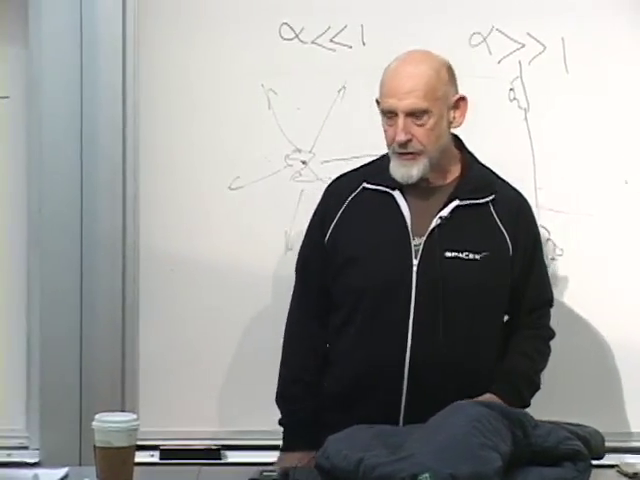
\includegraphics[width=0.72\textwidth]{lecture_01_figure_02.png}
\lectureframe{00:38:22.500}

\vspace{1em}

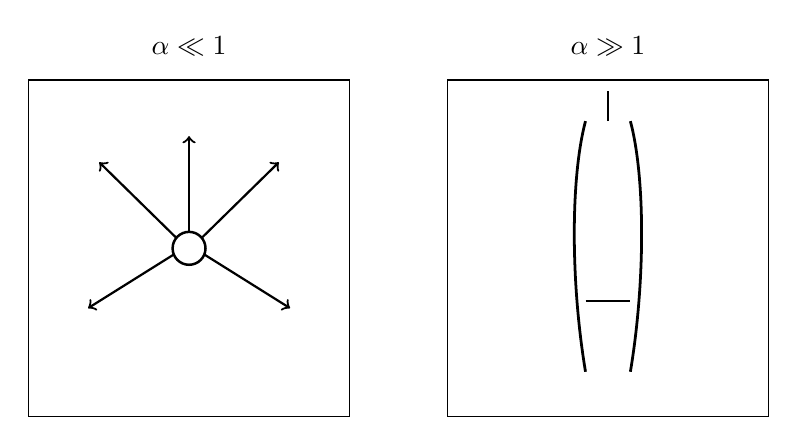
\begin{tikzpicture}[scale=0.95]
\draw (-5.3,-2.4) rectangle (-1.0,2.1);
\draw (0.3,-2.4) rectangle (4.6,2.1);

\node at (-3.15,2.55) {$\alpha \ll 1$};
\node at (2.45,2.55) {$\alpha \gg 1$};

\draw[line width=0.9pt] (-3.15,-0.15) circle (0.22);
\draw[->,line width=0.8pt] (-3.15,0.07) -- (-3.15,1.35);
\draw[->,line width=0.8pt] (-2.98,-0.01) -- (-1.95,1.00);
\draw[->,line width=0.8pt] (-3.32,-0.01) -- (-4.35,1.00);
\draw[->,line width=0.8pt] (-2.95,-0.23) -- (-1.80,-0.95);
\draw[->,line width=0.8pt] (-3.35,-0.23) -- (-4.50,-0.95);

\draw[line width=1.0pt] (2.15,-1.8) .. controls (1.95,-0.6) and (1.95,0.8) .. (2.15,1.55);
\draw[line width=1.0pt] (2.75,-1.8) .. controls (2.95,-0.6) and (2.95,0.8) .. (2.75,1.55);
\draw[line width=0.8pt] (2.15,-0.85) -- (2.75,-0.85);
\draw[line width=0.8pt] (2.45,1.55) -- (2.45,1.95);
\end{tikzpicture}
\caption{Сравнение слабой--сильной связи в КЭД в ходе обсуждения энергии взаимодействия. Диаграмма выделяет два режима, различимые в изложении Susskind: разрежённое облако при слабой связи и разрастающееся — при сильной.}
\end{figure}

Причина, по которой этот рисунок помещён именно здесь, хотя сравнение слабой--сильной связи было введено раньше, состоит в том, что в лекции Susskind заново проводит это противопоставление в этой более поздней, вызванной вопросом части, обсуждая энергию взаимодействия и разрастающуюся структуру.

\section{Теории с чётномерными бранами и возникающее дополнительное измерение}

До этого момента лекция выстраивала убедительный сюжет о взаимной замене: фермион против бозона, электрон против монополя, F-струна против D-струны. Следующий шаг ещё более удивителен. Susskind переходит к другой версии теории струн, с чётномерными D-бранами, а не с нечётномерными. Это различие существенно, потому что в этой теории нет D-струны, которую можно было бы обменять на F-струну. Здесь имеются D0-браны, D2-браны, D4-браны и так далее.

Поэтому предел сильной связи не может быть просто переименованием одной струны в другую. Согласно лекции, происходит нечто более странное: проявляется дополнительное пространственное измерение. Susskind намеренно сначала формулирует это в максимально драматической форме --- ``материализуется новое измерение'' ---, а затем сразу переводит это в более аккуратное утверждение: очень малое компактное направление расширяется, пока его уже нельзя игнорировать.

Этот учёт — часть самой идеи, поэтому он делает на нём паузу:
\begin{equation}
\begin{aligned}
10\text{-dimensional string theory} &= 9\text{ space}+1\text{ time},\\
11\text{-dimensional theory} &= 10\text{ space}+1\text{ time}.
\end{aligned}
\end{equation}
Согласно лекции, предел сильной связи теории с чётномерными бранами эффективно одиннадцатимерен.

\editorialnote{Теория с чётномерными бранами — это теория струн типа IIA, а её завершение при сильной связи — M-теория. В стандартных единицах радиус возникающей окружности и одиннадцатимерная планковская длина масштабируются как \(R_{11}=g_s\ell_s\) и \(\ell_{11}=g_s^{1/3}\ell_s\). Эти названия и формулы явно показывают современный словарь, стоящий за геометрическим изложением лекции.}

\subsection{Сэндвич с арахисовым маслом}

Чтобы наглядно представить компактное направление, Susskind использует модель ``сэндвича с арахисовым маслом'': две бесконечно тонкие ломтины хлеба, между которыми находится реальное пространство. Особое правило состоит в том, что выход через одну сторону возвращает на другую. В стандартном обозначении, которое в лекции описывается наглядно, а не формально, можно написать
\begin{equation}
y \sim y + 2\pi R.
\end{equation}
Если \(R\) очень мал, наблюдатели, живущие в этом сэндвиче, эффективно описывают свой мир как имеющий меньшую размерность. Тогда ключевое изменение при сильной связи таково:
\begin{equation}
g\uparrow
\qquad \Longrightarrow \qquad
R_{\mathrm{compact}}\uparrow.
\end{equation}
Вот что Susskind имеет в виду, когда говорит, что появляется новое измерение пространства: не то, что пространство создаётся из ничего, а то, что прежде крошечное компактное направление расширяется и становится видимым в эффективной теории.

\begin{figure}[htbp]
\centering
\resizebox{\linewidth}{!}{%
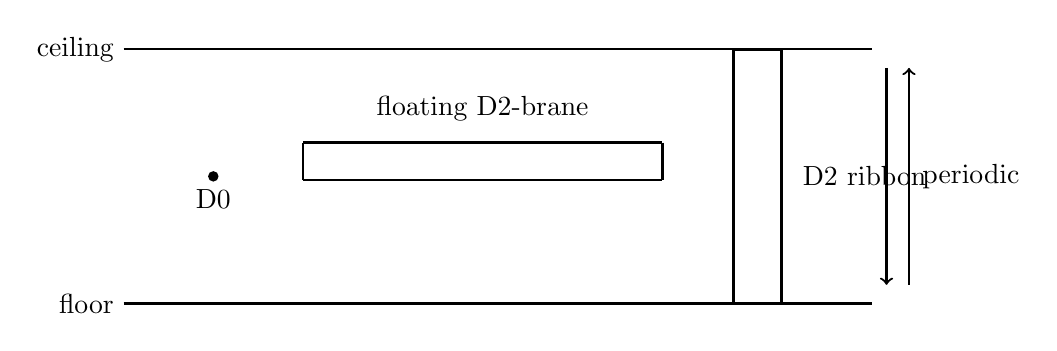
\begin{tikzpicture}[scale=0.95]
\draw[line width=0.9pt] (-5,1.7) -- (5,1.7);
\draw[line width=0.9pt] (-5,-1.7) -- (5,-1.7);

\node[left] at (-5,1.7) {ceiling};
\node[left] at (-5,-1.7) {floor};

\draw[->,line width=0.8pt] (5.2,1.45) -- (5.2,-1.45);
\draw[->,line width=0.8pt] (5.5,-1.45) -- (5.5,1.45);
\node[right] at (5.55,0) {periodic};

\draw[line width=1.0pt] (-2.6,0.45) -- (2.2,0.45);
\draw[line width=1.0pt] (-2.6,-0.05) -- (2.2,-0.05);
\draw[line width=1.0pt] (-2.6,0.45) -- (-2.6,-0.05);
\draw[line width=1.0pt] (2.2,0.45) -- (2.2,-0.05);
\node at (-0.2,0.9) {floating D2-brane};

\draw[line width=1.0pt] (3.15,-1.7) -- (3.8,-1.7);
\draw[line width=1.0pt] (3.15,1.7) -- (3.8,1.7);
\draw[line width=1.0pt] (3.15,-1.7) -- (3.15,1.7);
\draw[line width=1.0pt] (3.8,-1.7) -- (3.8,1.7);
\node[right] at (3.95,0) {D2 ribbon};

\fill (-3.8,0) circle (0.07);
\node[below] at (-3.8,-0.05) {D0};
\end{tikzpicture}
}%
\caption{Сэндвич-компактификация. Верхняя и нижняя границы периодически отождествляются; одна D2-брана парит между ними, как ковёр, а другая тянется от пола до потолка и выглядит струнообразной, когда компактное направление мало.}
\end{figure}

\subsection{Что происходит с D0- и D2-бранами?}

Теперь в лекции ставится вопрос о том, что происходит с D0-бранами и струнами. Ответ несимметричен. По мере роста \(g\) D0-браны делаются всё легче и легче; в более высокоразмерной интерпретации они входят в башню частиц, несущих импульс во вновь проявившемся направлении. Тем самым тяжёлый, сложный объект в картине слабой связи становится обычным лёгким возбуждением в картине сильной связи.

Соотношение масс показывает это отождествление:
\begin{equation}
M_{D0}(n)=\frac{n}{g_s\ell_s}
=\frac{n}{R_{11}}
=M_{\mathrm{KK}}(n).
\end{equation}
\editorialnote{Susskind называет D0-браны ``гравитонами'' одиннадцатимерной теории. Точнее, их связанные состояния — это моды импульса Калуцы--Клейна мультиплета одиннадцатимерной супергравитации, безмассовый сектор которого содержит гравитон. Это различие сохраняет физическое отождествление из лекции, избегая при этом слишком буквального утверждения на уровне одной частицы.}

D2-браны объясняют судьбу струн. В лекции выделены две конфигурации:
\begin{enumerate}
\item D2-брана, плавающая между полом и потолком, как ковёр в арахисовом масле;
\item D2-брана, натянутая от пола до потолка, как лента, и протянутая вдоль видимого направления.
\end{enumerate}
Когда сэндвич тонок, лента выглядит эффективно одномерной. Это тот объект, который наблюдатели низких энергий называют струной. По мере того как компактное направление раскрывается, тот же самый объект становится несомненно мембраноподобным. Поскольку теперь в вертикальном направлении в нём больше материала, он становится тяжёлым и уже не похожим на струну.

\paragraph{Логика перехода.}
\begin{enumerate}
\item Начните с очень тонкого компактного направления, так что лента от пола до потолка эффективно ведёт себя как струна.
\item С увеличением \(g\) компактное направление расширяется.
\item D0-браны становятся лёгкими и переинтерпретируются как состояния импульса Калуцы--Клейна в более высокоразмерной теории.
\item Струноподобная D2-лента становится явно протяжённой мембраной и тяжелеет.
\end{enumerate}
Это узловой переход лекции от дуальности к возникающей геометрии. Сильная связь не просто обменивает один объект на другой; она меняет то, какая геометрия является эффективной.

Susskind останавливается на том, насколько странно это звучит. Сеть предлагаемых отождествлений требовала трудных математических соотношений согласованности; некоторые из них сначала появились у физиков как гипотезы, а позднее были доказаны математиками. Он не утверждает, что каждый реалистический вакуум теории струн понят, но утверждает, что сама сеть дуальностей выдержала необычайно жёсткие проверки.

Если в этой идеализированной постановке константа связи меняется от места к месту, вместе с ней может меняться и эффективная геометрия. Одна область может выглядеть почти десятимерной, с лёгкими струнами и тяжёлыми D0-бранами; другая может раскрываться в одиннадцатимерное описание, с тяжёлыми обёрнутыми мембранами и лёгкими модами Калуцы--Клейна. Локальная смена языка описания — часть той же самой сети дуальностей.

Стенограмма кратко передаёт название этих соотношений как ``неравенства.'' По контексту имеется в виду слово \emph{дуальности}: связи между противоположными концами пространства параметров. Эта поправка важна, потому что вывод лекции как раз и состоит в том, что никакого единственного списка фундаментальных составляющих не известно. Струны, браны, частицы и геометрия более высоких измерений могут переходить друг в друга; либо ни один элемент этой сети не является абсолютно фундаментальным, либо какая-то более глубокая организация остаётся неизвестной.

\section{D3-браны, обёрнутые мембраны и геометрическая картина дуальности}

После перерыва Susskind прямо описывает эту тему как ``огромную сеть'' взаимосвязанных теорий и идей. Следующие примеры — это не новые изолированные эффекты; это мосты, связывающие предыдущие.

\subsection{Мировой объём D3-браны}

В первом мосте используется D3-брана. D3-брана имеет три пространственных измерения, и наблюдатель, ограниченный ею, легко может принять ее за обычное пространство. Брана может изгибаться и флуктуировать, а струны, оканчивающиеся на ней, могут соединяться, расщепляться и рассеиваться. Для наблюдателя, видящего только направления вдоль браны, каждый конец выглядит как частица, а взаимодействия между концами выглядят как обычная квантовая теория поля.

\begin{figure}[htbp]
\centering
\resizebox{\linewidth}{!}{%
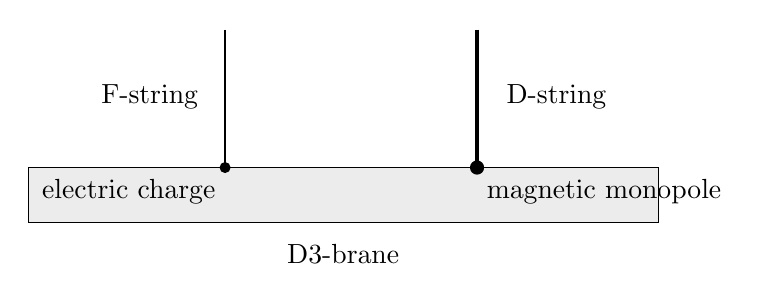
\begin{tikzpicture}[scale=1.0]
\draw[fill=gray!15] (-4,-0.35) rectangle (4,0.35);
\node at (0,-0.75) {D3-brane};

\draw[line width=0.9pt] (-1.5,2.1) -- (-1.5,0.35);
\fill (-1.5,0.35) circle (0.07);
\node[left] at (-1.72,1.25) {F-string};
\node[below left] at (-1.5,0.32) {electric charge};

\draw[line width=1.5pt] (1.7,2.1) -- (1.7,0.35);
\fill (1.7,0.35) circle (0.09);
\node[right] at (1.95,1.25) {D-string};
\node[below right] at (1.7,0.32) {magnetic monopole};
\end{tikzpicture}
}%
\caption{Интерпретация на мировом объеме D3-браны. Конец F-струны выглядит как электрический заряд; конец D-струны — как магнитный монополь.}
\end{figure}

Это одно из самых удачных отождествлений в лекции. F-струна, оканчивающаяся на D3-бране, выглядит для наблюдателя на мировом объеме как электрический заряд. D-струна, оканчивающаяся на той же бране, выглядит как магнитный монополь. Иными словами, дуальность между F-струнами и D-струнами на мировом объеме D3-браны становится электрическо--магнитной дуальностью обычной теории поля. То, что раньше было аналогией, теперь стало явным словарем соответствий.

\editorialnote{Для стопки D3-бран низкоэнергетическое описание на мировом объеме представляет собой четырехмерную \(\mathcal N=4\) суперсимметричную теорию Янга--Миллса. Ее электрическо--магнитная дуальность является реализацией S-дуальности теории типа IIB на языке теории поля; одиночная брана дает абелев предел, использованный в лекции для наглядности.}

\subsection{Два компактных направления и асимметричное обертывание}

Затем Susskind возвращается к многомерной геометрии и компактифицирует не одно, а два малых направления. Поскольку изобразить на доске 11 измерений невозможно, он сжимает 7 больших направлений, не использованных в схеме, в одно видимое горизонтальное направление, а затем явно рисует два компактных. Он настаивает на асимметричном изображении компактификации, потому что одно компактное направление должно быть короче другого, если эффективные струны должны иметь разные натяжения.

\begin{figure}[htbp]
\centering
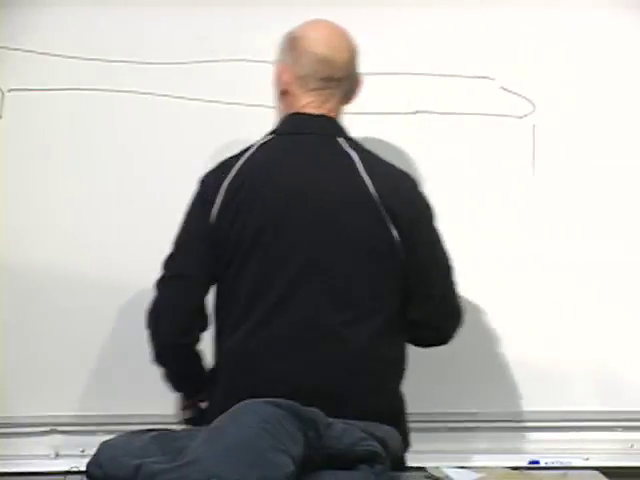
\includegraphics[width=0.78\textwidth]{lecture_01_figure_03.png}
\lectureframe{01:10:25.000}
\caption{Окончательный рисунок на доске для двух обернутых мембран. Короткий и длинный компактные циклы дают показанные справа ленты, подобные F- и D-струнам.}
\end{figure}

Мембрана может обертывать любое из компактных направлений и из некомпактных направлений выглядеть как струна. Если \(R_1\) и \(R_2\) — это два радиуса окружностей, то ее эффективные натяжения равны
\begin{equation}
\begin{aligned}
T_{(1)}&=2\pi R_1 T_{\mathrm{M2}},\\
T_{(2)}&=2\pi R_2 T_{\mathrm{M2}},\\
\frac{T_{(1)}}{T_{(2)}}&=\frac{R_1}{R_2}.
\end{aligned}
\end{equation}
Таким образом, неодинаковые размеры окружностей дают неодинаковые натяжения струн. Если отождествить более короткое обертывание с легкой F-струной, а более длинное — с тяжелой D-струной, то схематически можно написать
\begin{equation}
g_s\sim \frac{R_{\mathrm{short}}}{R_{\mathrm{long}}},
\qquad
\frac{T_{\mathrm{D1}}}{T_{\mathrm{F1}}}\sim \frac{1}{g_s}.
\end{equation}

\begin{classroomqa}
\audiencequestion{Можно ли в этой картине понимать константу связи как отношение двух компактных размеров? \lecturetimestamp{01:10:13}}
\lecturerresponse{Да. Параметр слабо--сильной связи геометризуется как отношение сторон. Если сделать одно направление коротким, константа связи станет малой; если поменять два направления местами, легкая и тяжелая струны поменяются ролями.}
\end{classroomqa}

\editorialnote{В лекции это отношение временно обозначается через \(\alpha\), то есть повторно используется символ, ранее употреблявшийся для постоянной тонкой структуры КЭД. Здесь мы пишем \(g_s\), чтобы различать эти два значения. В полном построении M-теории константа связи типа IIB кодируется комплексной структурой компактного двумерного тора; точный числитель зависит от того, как помечены его циклы.}

Картину с обернутыми мембранами можно подытожить без перспективных искажений рисунка на доске:

\begin{figure}[htbp]
\centering
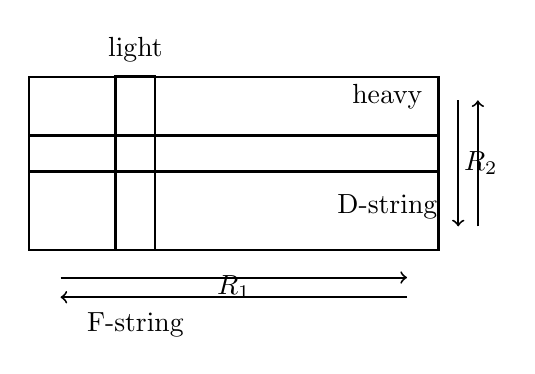
\begin{tikzpicture}[scale=1.0]
\draw[line width=0.9pt] (0,0) rectangle (5.2,2.2);
\node[below] at (2.6,-0.2) {\(R_1\)};
\node[right] at (5.4,1.1) {\(R_2\)};

\draw[->,line width=0.7pt] (5.45,1.9) -- (5.45,0.3);
\draw[->,line width=0.7pt] (5.7,0.3) -- (5.7,1.9);
\draw[->,line width=0.7pt] (0.4,-0.35) -- (4.8,-0.35);
\draw[->,line width=0.7pt] (4.8,-0.6) -- (0.4,-0.6);

\draw[line width=1.0pt] (1.1,0) -- (1.6,0) -- (1.6,2.2) -- (1.1,2.2) -- cycle;
\node at (1.35,2.55) {light};

\draw[line width=1.0pt] (0,1.45) -- (5.2,1.45);
\draw[line width=1.0pt] (0,1.00) -- (5.2,1.00);
\node at (4.55,1.95) {heavy};

\node at (1.35,-0.95) {F-string};
\node at (4.55,0.55) {D-string};
\end{tikzpicture}
\caption{Обе конфигурации обернутой мембраны из некомпактных направлений выглядят как струны, но из-за неравных компактных масштабов одна эффективная струна оказывается легче другой.}
\end{figure}

Это геометрическая версия прежнего сюжета о дуальности. Сжатие одного направления при растяжении другого делает один обернутый объект тяжелее, а другой легче, так что роли F-струны и D-струны могут меняться местами.

\begin{classroomqa}
\audiencequestion{Если компактные направления циклические, не становятся ли обернутые объекты бесконечно широкими? \lecturetimestamp{01:10:41}}
\lecturerresponse{Нет. Компактная окружность имеет конечную длину, хотя по ней можно проходить снова и снова, не достигая края. Верх и низ разрезанного рисунка представляют одну и ту же точку, так же как концы интервала могут представлять одну точку окружности.}
\end{classroomqa}

\begin{figure}[htbp]
\centering
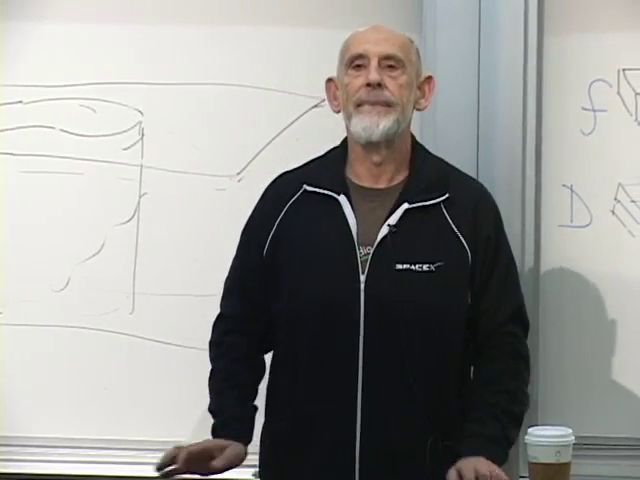
\includegraphics[width=0.78\textwidth]{lecture_01_figure_04.png}
\lectureframe{01:12:25.000}

\vspace{1em}

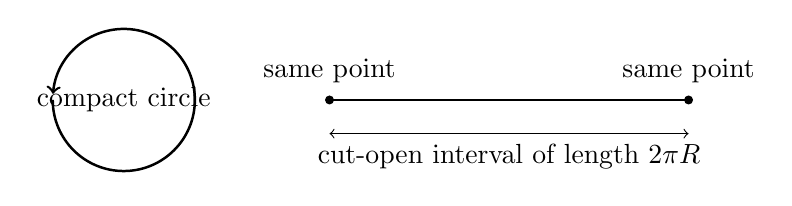
\begin{tikzpicture}[scale=0.95]
\draw[line width=0.9pt,->] (-3.7,0) arc[start angle=180,end angle=535,radius=0.95];
\node at (-2.75,0) {compact circle};
\draw[line width=0.9pt] (0.0,0) -- (4.8,0);
\fill (0.0,0) circle (0.06);
\fill (4.8,0) circle (0.06);
\draw[<->] (0.0,-0.45) -- (4.8,-0.45);
\node at (2.4,-0.75) {cut-open interval of length \(2\pi R\)};
\node[above] at (0.0,0.1) {same point};
\node[above] at (4.8,0.1) {same point};
\end{tikzpicture}
\caption{Компактная окружность и ее разрезанное изображение на доске. Переход через один конец возвращает к другому; движение по окружности при одновременном движении в некомпактном направлении дало бы вместо этого винтовую линию.}
\end{figure}

\begin{classroomqa}
\audiencequestion{Почему компактный путь — это окружность, а не винтовая линия? \lecturetimestamp{01:12:23}}
\lecturerresponse{В каждой фиксированной точке некомпактного направления компактное направление является окружностью. Винтовая линия появляется только тогда, когда движение по некомпактному направлению сопровождается одновременной намоткой вокруг окружности. Интервал на доске — это просто разрезанная окружность с отождествленными концами.}
\end{classroomqa}

\begin{classroomqa}
\audiencequestion{Объясняет ли сама эта геометрия, как D-брана при достаточно детальном зондировании может выглядеть как набор F-струн? \lecturetimestamp{01:12:49}}
\lecturerresponse{Связь здесь есть, но в этой элементарной картине она не прозрачна; чтобы ее увидеть, нужен более развитый геометрический аппарат. Диаграмма предназначена для организации дуальности, а не для вывода всякого описания на уровне микроскопических составляющих.}
\end{classroomqa}

\begin{classroomqa}
\audiencequestion{Могут ли длинное и короткое компактные направления меняться местами при перемещении в пространстве или по мере эволюции во времени? \lecturetimestamp{01:13:35}}
\lecturerresponse{В идеализированной модели возможно и то и другое. Если сжать один цикл и расширить другой, то меняется, какая из обернутых струн является легкой. Это еще одна причина, почему ``фундаментальная струна'' — лишь название: предпочтительное описание может меняться от области к области или со временем.}
\end{classroomqa}

\section{Идеализация, особо симметричные точки и ландшафт}

В последней части лекции делается шаг назад от изящных примеров дуальности и ставится вопрос о том, что они говорят, и чего не говорят, о реальном мире.

Сначала Susskind предупреждает, что точно контролируемые дуальности являются свойствами сильно идеализированных суперсимметричных теорий, в которых бозоны и фермионы имеют в точности совпадающие массы. В качестве аналогии он приводит круговые орбиты в ньютоновской механике: их сначала изучают потому, что они симметричны и математически удобны, а не потому, что реальное движение планет исчерпывается идеальными окружностями. Точно так же суперсимметричные теории струн легче анализировать, потому что они более симметричны, чем, по-видимому, природа.

Тем не менее такая идеализация поучительна. Идеально круговая орбита не является реалистической планетной системой, но она демонстрирует черты, сохраняющиеся и в менее симметричных орбитах. Аналогично, суперсимметричные примеры показывают непротиворечивые способы, которыми квантовая механика, гравитация и микроскопическая структура могут согласованно сочетаться. Намеренно заостренная формулировка Susskind состоит в том, что теории струн, поддающиеся анализу, не являются в буквальном смысле теорией нашего мира; их ценность в том, что они выявляют явления, которые, вероятно, снова появятся в менее симметричных и менее податливых для анализа ситуациях.

\subsection{Конструктор с множеством вариантов}

D-браны — лишь часть доступного набора строительных элементов. В лекции также упоминаются потоки, орбифолды и ориентifoldы. Сначала выбирают компактную геометрию, затем — какие браны и потоки размещаются на ее циклах. Даже простой сэндвич меняет свою физику в меньшем числе измерений, если вставить в него одну плавающую D2-брану, две или три. Добавление или удаление таких ингредиентов меняет эффективные частицы, взаимодействия и параметры.

Предположим, что в схематическом подсчете, приведенном в лекции, шестимерное компактное пространство имеет примерно \(500\) циклов и каждый цикл допускает порядка \(10\) вариантов обернутых бран, потоков или родственных структур. Тогда число конструкций растет как
\begin{equation}
N_{\mathrm{vacua}} \sim 10^{500}.
\end{equation}
Логика подсчета в лекции элементарна:
\begin{equation}
10 \times 10 \times \cdots \times 10 = 10^{500}
\end{equation}
с \(500\) множителями. Аналогия с ДНК выражает ту же мысль в более привычном виде:
\begin{equation}
N_{\mathrm{DNA}}(500)=4^{500}.
\end{equation}
Во время сравнения с ДНК один из слушателей уточняет, что вдоль одной цепочки есть четыре возможности: A, C, G и T. Эта поправка скорее усиливает аргумент, чем меняет его. Короткий список локальных выборов, многократно повторенный, порождает огромное число глобальных конфигураций. Точное значение показателя несущественно, и Susskind называет \(10^{500}\) старой заниженной оценкой; существенна комбинаторная пролиферация.

Это дает последний переворот исходного редукционистского ожидания. Сложная физика частиц не обязана возникать из сложных микроскопических правил. Она может возникать потому, что наш вакуум представляет собой одну сложную конфигурацию из многих простых ингредиентов, точно так же как сложный организм может кодироваться последовательностью, построенной из четырех оснований.

\begin{classroomqa}
\audiencequestion{После отождествления эквивалентных описаний, связанных дуальностью, выделила бы полная информация только один или несколько из этих возможных вакуумов в качестве описаний нашего мира? \lecturetimestamp{01:26:11}}
\lecturerresponse{Предположительно, она выделила бы ограниченное множество, но многие различные вакуумы могут выглядеть чрезвычайно похожими при доступных энергиях. Приводимая оценка числа ландшафта должна оставаться большой даже после отождествления дуальных описаний, а несущественные высокоэнергетические детали могут функционировать как ``мусорная ДНК.''}
\end{classroomqa}

\subsection{Симметричные точки и типичная сложность}

В ландшафте имеются точки с особой симметрией. В геометрической картине конфигурация с равными размерами,
\begin{equation}
R_1=R_2,
\end{equation}
делает оба описания через обёрнутые струны одинаково простыми. В электрической--магнитной аналогии это схематически выражается как
\begin{equation}
m_{\mathrm{monopole}}=m_e.
\end{equation}

\begin{figure}[htbp]
\centering
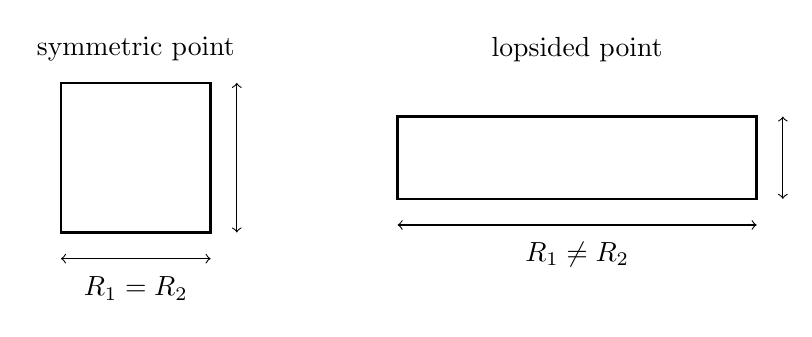
\begin{tikzpicture}[scale=0.95]
\draw[line width=0.9pt] (-4.5,-1.0) rectangle (-2.5,1.0);
\draw[<->] (-4.5,-1.35) -- (-2.5,-1.35);
\draw[<->] (-2.15,-1.0) -- (-2.15,1.0);
\node at (-3.5,1.45) {symmetric point};
\node at (-3.5,-1.75) {$R_1=R_2$};

\draw[line width=0.9pt] (0.0,-0.55) rectangle (4.8,0.55);
\draw[<->] (0.0,-0.9) -- (4.8,-0.9);
\draw[<->] (5.15,-0.55) -- (5.15,0.55);
\node at (2.4,1.45) {lopsided point};
\node at (2.4,-1.3) {$R_1\ne R_2$};
\end{tikzpicture}
\caption{При компактификации с равными размерами две обёрнутые струны трактуются симметрично; при перекошенной компактификации одно описание становится намного легче другого.}
\end{figure}

\begin{classroomqa}
\audiencequestion{Существуют ли в ландшафте вакуумы, в которых конструкция становится намного проще, потому что описания через F- и D-струны совпадают? \lecturetimestamp{01:27:21}}
\lecturerresponse{Да, существуют особо симметричные точки. Наш мир, по-видимому, не находится в одной из них: у известной электрической частицы и магнитного монополя массы не равны. Почему природа находится в перекошенной точке, неизвестно.}
\end{classroomqa}

\editorialnote{Электрон--монопольное равенство масс — это схематическая черта должным образом защищённой самодуальной модели, а не предсказание обычной несуперсимметричной КЭД. Оно выражает обсуждаемую в лекции идею симметричной точки, а не утверждение о наблюдаемом электроне.}

Сасскинд затем вспоминает аналогию из теории связи. Случайные коды могут быть необычайно хороши, тогда как коды, которые легче всего описывать и декодировать, обладают дополнительной математической структурой и исторически показывали худшие результаты. Позднее теория кодирования нашла весьма эффективные структурированные конструкции, но аналогия сохраняется: всё, что можно кратко назвать или описать, занимает в полном пространстве возможностей очень особый угол малой сложности. Точно так же струнные вакуумы, которые легче всего вычислять, могут быть нетипично простыми.

Поэтому сами уместные вопросы могут измениться. Вместо того чтобы требовать точную компактификацию во всех микроскопических деталях, можно спрашивать, какие свойства являются общими или типичными в широком ансамбле. Сасскинд представляет это как исследовательскую задачу, а не как окончательный вывод, и отвергает подмену вычислений идеологическими доводами.

\subsection{Космологические вопросы}

\begin{classroomqa}
\audiencequestion{Наблюдательно отличимо ли компактное направление с огромной длиной окружности от бесконечного направления, и знаем ли мы, что наши три большие пространственные измерения бесконечны? \lecturetimestamp{01:30:03}}
\lecturerresponse{Мы не знаем, что они бесконечны. Замкнутая трёхсфера может расширяться, оставаясь компактной. Измерения близости к плоскости дают лишь нижнюю границу на радиус кривизны, подобно тому как съёмка почти плоского поля может дать нижнюю границу на размер Земли, не доказывая, что её поверхность бесконечна. Только обнаруженная кривизна или глобальное отождествление позволили бы определить конечный масштаб.}
\end{classroomqa}

\begin{classroomqa}
\audiencequestion{Если константа связи в идеализированной модели может меняться в пространстве, то как такое изменение могло бы происходить в реальном мире? \lecturetimestamp{01:32:43}}
\lecturerresponse{Не в виде неограниченного гладкого изменения, использованного в симметричном примере. Реалистическая возможность, о которой пойдёт речь позже, — это изменение через дискретные переходы между областями с различными эффективными законами. Вопрос о том, происходят ли такие скачки, является космологическим.}
\end{classroomqa}

\editorialnote{Этот ответ следует читать как предваряющее упоминание в лекции о флюкс-вакуумах и переходах между доменами, а не как общую теорему, запрещающую всякое гладко меняющееся скалярное поле. Наблюдения сильно ограничивают вариации безразмерных констант связи, тогда как механизмы стабилизации определяют, остаются ли в данной модели доступными непрерывные модули.}

Запись не сохранила последний вопрос из аудитории. Сохранившийся ответ говорит, что предложенное явление может происходить для некоторых видов чёрных дыр, но не на горизонте обычной чёрной дыры Шварцшильда, горизонт которой локально является обычным местом для свободно падающего наблюдателя. Поскольку вопрос нельзя надёжно восстановить, этому обмену репликами не приписывается никакого более конкретного утверждения.

\section{От кирпичиков к сети описаний}

Надежда на то, что более глубокие слои физики должны быть проще, оказалась непрочной. В бозонизации в \(1+1\) измерениях одну и ту же теорию можно организовать либо как описание через фермионы, либо как описание через бозоны, причём фермион вновь появляется как кинк. В квантовой электродинамике режимы слабой и сильной связи меняют местами описательные роли электрона и магнитного монополя. В теории струн F-струны и D-струны повторяют ту же схему, а в теории чётных бран при сильной связи дело заходит ещё дальше: компактное направление расширяется, D0-браны становятся состояниями импульса Калуцы--Клейна, а эффективные струны переинтерпретируются как обёрнутые мембраны в геометрии более высокой размерности. Поэтому современная квантовая теория поля и теория струн не дают единственного, раз и навсегда установленного ответа на вопрос ``что здесь кирпичики, а что дома?'' Они дают сеть описаний, каждое эффективное в своём собственном режиме, вместе с огромным ландшафтом возможных конструкций, типичным результатом которого является сложность, а не простота.
